\chapter{Methodology}%
\label{chapter:methodology}

\begin{introduction}
This chapter presents the non-functional requirements and the use cases of the applications. 
\end{introduction} 




\section{Applications Requirements} 


To identify the requirements of the application, I used the FURPS model. 
The non-functional requirements are listed below:

\begin{itemize}
  \item Scalability – The system should be able to support users from Europe.
  \item Reliability – The system should have a high availability of 99\% and the system also should not take longer than 4 hours to recover from a failure.
  \item Performance – The system should not take longer than 2 seconds to respond.
  \item Usability – The train of a new user should not take longer than 8 hours.
  \item Supportability – The system should be supported on the web browsers Chrome, Firefox, Microsoft Edge, and Safari.
\end{itemize}

For the functional requirements of the applications, I developed a set of use cases for each user.
As mentioned in Chapter II, the dealership application is structured into four key user roles: receptionist, mechanic, warehouse operator, and administrator.

The receptionist will be responsible for interacting with the client, this includes the vehicle check-in and check-out and user communication. 
The use cases are:

\begin{itemize}
    \item Use Case 1.1 – Vehicle Reception
    \begin{itemize}
      \item Scenario – The client arrives at the dealership with a vehicle to be repaired.
      \item Objective – Create a new maintenance request in the system.
      \item System – The receptionist inserts in the form all the information about the initial maintenance request from the client and creates a new maintenance request with the date and budget agreed upon by him 
    \end{itemize}
    \item Use Case 1.2 – Vehicle Delivery 
    \begin{itemize}
      \item Scenario – The Receptionist delivered the vehicle to the Client.
      \item Objective – Complete the vehicle maintenance process.
      \item System – Sends a report in a PDF format to the client with the information about the maintenance and alters the maintenance request status in the system to conclude. 
    \end{itemize}
    \item Use Case 1.3 – Collect information about a maintenance request
    \begin{itemize}
      \item Scenario – A Client calls the dealership to ask about the maintenance of his vehicle.
      \item Objective – Visualize the maintenance information.
      \item System –  The Receptionist searches a list of maintenance requests by vehicle/customer or name/maintenance ID and he can visualize the maintenance details of a specific item.
    \end{itemize}
    \item Use Case 1.4 – Asking for customer permission
    \begin{itemize}
      \item Scenario – A problem in a vehicle maintenance has occurred and the initial agreement with the client may be broken.
      \item Objective – Inform the client of the problem and achieve an agreement.
      \item System – The Receptionist receives an alert that there has been a change in the initial maintenance budget and/or completion deadline, so he needs to contact the customer to inform him. Depending on customer feedback, the receptionist accepts the maintenance request, declines the maintenance request, or terminates the maintenance.
    \end{itemize}
  \end{itemize}  
  \hfill \break


 The mechanic will be responsible for doing the maintenance in the vehicle, like oil change, tire change, trade vehicle parts, etc. 
 It will previously evaluate the vehicle and after the maintenance is done, it will write a report of the operations done. 
 The mechanic use cases are:

  \begin{itemize}
    \item Use Case 2.1 – View to-do list
    \begin{itemize}
      \item Scenario – The mechanic arrives at the dealership and wants to see what tasks he has to do today.
      \item Objective – See the day's work organization.
      \item System – The mechanic watches a list of tasks that were assigned from the administrator, as soon as he enters the system. Each task is accompanied by a description, a priority, a vehicle identification, a set of actions to be performed, and comments from other users. 
    \end{itemize}
    \item Use Case 2.2 – Carry out a vehicle analysis 
    \begin{itemize}
      \item Scenario – A new vehicle needs to be analyzed.
      \item Objective – Confirm the initial analysis of the receptionist and search for additional problems.
      \item System – The mechanic enters the problems he finds in the vehicle into the system. 
    \end{itemize}
    \item Use Case 2.3 – Prepare a list of necessary parts
    \begin{itemize}
      \item Scenario – After vehicle analysis.
      \item Objective – Elaborate a request for vehicle parts to the warehouse.
      \item System – The mechanic selects the parts of the vehicle that need to be replaced and sends a request with the new parts to the warehouse.
    \end{itemize}
    \item Use Case 2.4 – Collect the requested parts in the Warehouse
    \begin{itemize}
      \item Scenario – The mechanic goes to the warehouse to collect new parts for the vehicle.
      \item Objective – Collect parts to replace the damaged parts in the vehicle.
      \item System – The mechanic adds the new parts to the vehicle in the system.
    \end{itemize}
    \item Use Case 2.5 – Deliver damaged parts to the Warehouse
    \begin{itemize}
      \item Scenario – The mechanic goes to the warehouse to deliver the damaged parts.
      \item Objective – Register the damaged parts.
      \item System – The mechanic removes the damaged parts from the vehicle and changes the status to damaged.
    \end{itemize}
\item Use Case 2.6 – Vehicle maintenance
\begin{itemize}
  \item Scenario – A new vehicle is ready for maintenance.
  \item Objective – The mechanic will do the vehicle maintenance (oil change, tire change, vehicle wash…).
  \item System – The mechanic sees a set of tasks that he needs to do to complete the vehicle maintenance and whenever he finishes a task, he marks it as completed.
\end{itemize}
\item Use Case 2.7 – Making the repair report
\begin{itemize}
  \item Scenario – After vehicle maintenance.
  \item Objective – Conclude the maintenance of a vehicle.
  \item System – The Mechanic enters into the system all operations and tests carried out on the system as well as their results.
\end{itemize}
\end{itemize}
\hfill \break

The warehouse operator is responsible for managing the dealer's stock and asking for supplies. 
In this case, the use cases are as follows:

\begin{itemize}
  \item Use Case 3.1 – View the different parts that the warehouse possess
  \begin{itemize}
    \item Scenario – The warehouse worker wants to view the quantity of certain parts that the warehouse possesses.
    \item Objective – Show quantitative warehouse information.
    \item System – List of all parts and their quantities that the warehouse possesses. 
  \end{itemize}
  \item Use Case 3.2 – Requesting purchasing service 
  \begin{itemize}
    \item Scenario – The warehouse worker discovers that he has an insufficient number of parts for maintenance or anticipates that this part will be missing soon.
    \item Objective – Request permission to purchase parts from the supplier.
    \item System – The Warehouse Worker will place a purchase order for parts. The system notifies the administrator via the platform and by email requesting authorization to make the purchase. 
  \end{itemize}
  \item Use Case 3.3 – Registration of new parts in the System
  \begin{itemize}
    \item Scenario – The warehouse purchased several parts from a supplier.
    \item Objective – Register new parts in the system.
    \item System – The warehouse operator adds a specific type of part to the system with its appropriate description and identification.
  \end{itemize}
\end{itemize}
\hfill \break

The last user of the application is the administrator or Workshop Manager. This user is in charge of managing the platform and the dealership. So the main use cases encountered are:

\begin{itemize}
  \item Use Case 4.1 – Authorizing purchases
  \begin{itemize}
    \item Scenario –  The administrator received a purchase request.
    \item Objective – Authorize or reject a purchase authorization request.
    \item System – List of all purchase authorization requests, as well as their details. The administrator can change the status of this request, rejecting or authorizing it. 
  \end{itemize}
  \item Use Case 4.2 – View history of maintenance performed
  \begin{itemize}
    \item Scenario – The administrator wants to gather information from recently performed maintenance.
    \item Objective – View information about a specific maintenance that occurred.
    \item System – List of all maintenance that occurred as well as its details (who carried it out, which parts were removed, the name of the customer, tests carried out, and their results…). 
  \end{itemize}
  \item Use Case 4.3 – Develop statistics
  \begin{itemize}
    \item Scenario – The administrator wants to gather statistics on the maintenance that was carried out in the last month.
    \item Objective – View information about maintenance over a given period of time.
    \item System – Presentation graphs of the number of parts replaced, number of purchases, total price spent on new parts, remuneration for maintenance, average customer rating, etc.
  \end{itemize}
  \item Use Case 4.4 – Assign roles to employees
  \begin{itemize}
    \item Scenario – A new employee has been hired.
    \item Objective –  Assign roles to new employees.
    \item System – The administrator assigns to the new employee a certain role and set of permissions.
  \end{itemize}
  \item Use Case 4.5 – Assign tasks to the employees
  \begin{itemize}
    \item Scenario – A new maintenance request has been requested.
    \item Objective – Assign and organize tasks to different employees.
    \item System – The administrator assigns the various tasks of vehicle maintenance to the workshop employees.
  \end{itemize}
\end{itemize}
\hfill \break

The client application will only be interacted with by a role of users, the client.
The use cases are listed below:

\begin{itemize}
  \item Use Case 5.1 – View current maintenance status
  \begin{itemize}
    \item Scenario – The Customer wants to find information regarding the vehicle maintenance procedure.
    \item Objective – Display current maintenance status.
    \item System – The system will illustrate all the maintenance steps that the vehicle has already undergone, as well as those that remain to be completed. 
  \end{itemize}
  \item Use Case 5.2 – Notify the customer of the end of maintenance 
  \begin{itemize}
    \item Scenario – Vehicle maintenance has been completed and the customer can now collect the vehicle.
    \item Objective – Notify the user of the end of maintenance.
    \item System – The system will show an SMS/native notification on the customer's cell phone informing that the vehicle is ready to be picked up. 
  \end{itemize}
  \item Use Case 5.3 – Rating of the service provided
  \begin{itemize}
    \item Scenario – The client receives the vehicle and the receptionist completes the maintenance process.
    \item Objective – Get feedback from the client.
    \item System – The system will show a form to the client asking about the service provided. 
  \end{itemize}
\end{itemize}
\hfill \break

\section{Applications Workflow}

After the development of the use cases, a flow chart was designed to understand the users' interaction with the system and each other. The chart is visible in figure \ref{fig:figure2}.

\begin{figure}[h]
  \caption{Use Case Flow Chart of the Client, Receptionist, Mechanic, Warehouse Operator, and Administrator.}
  \centering
  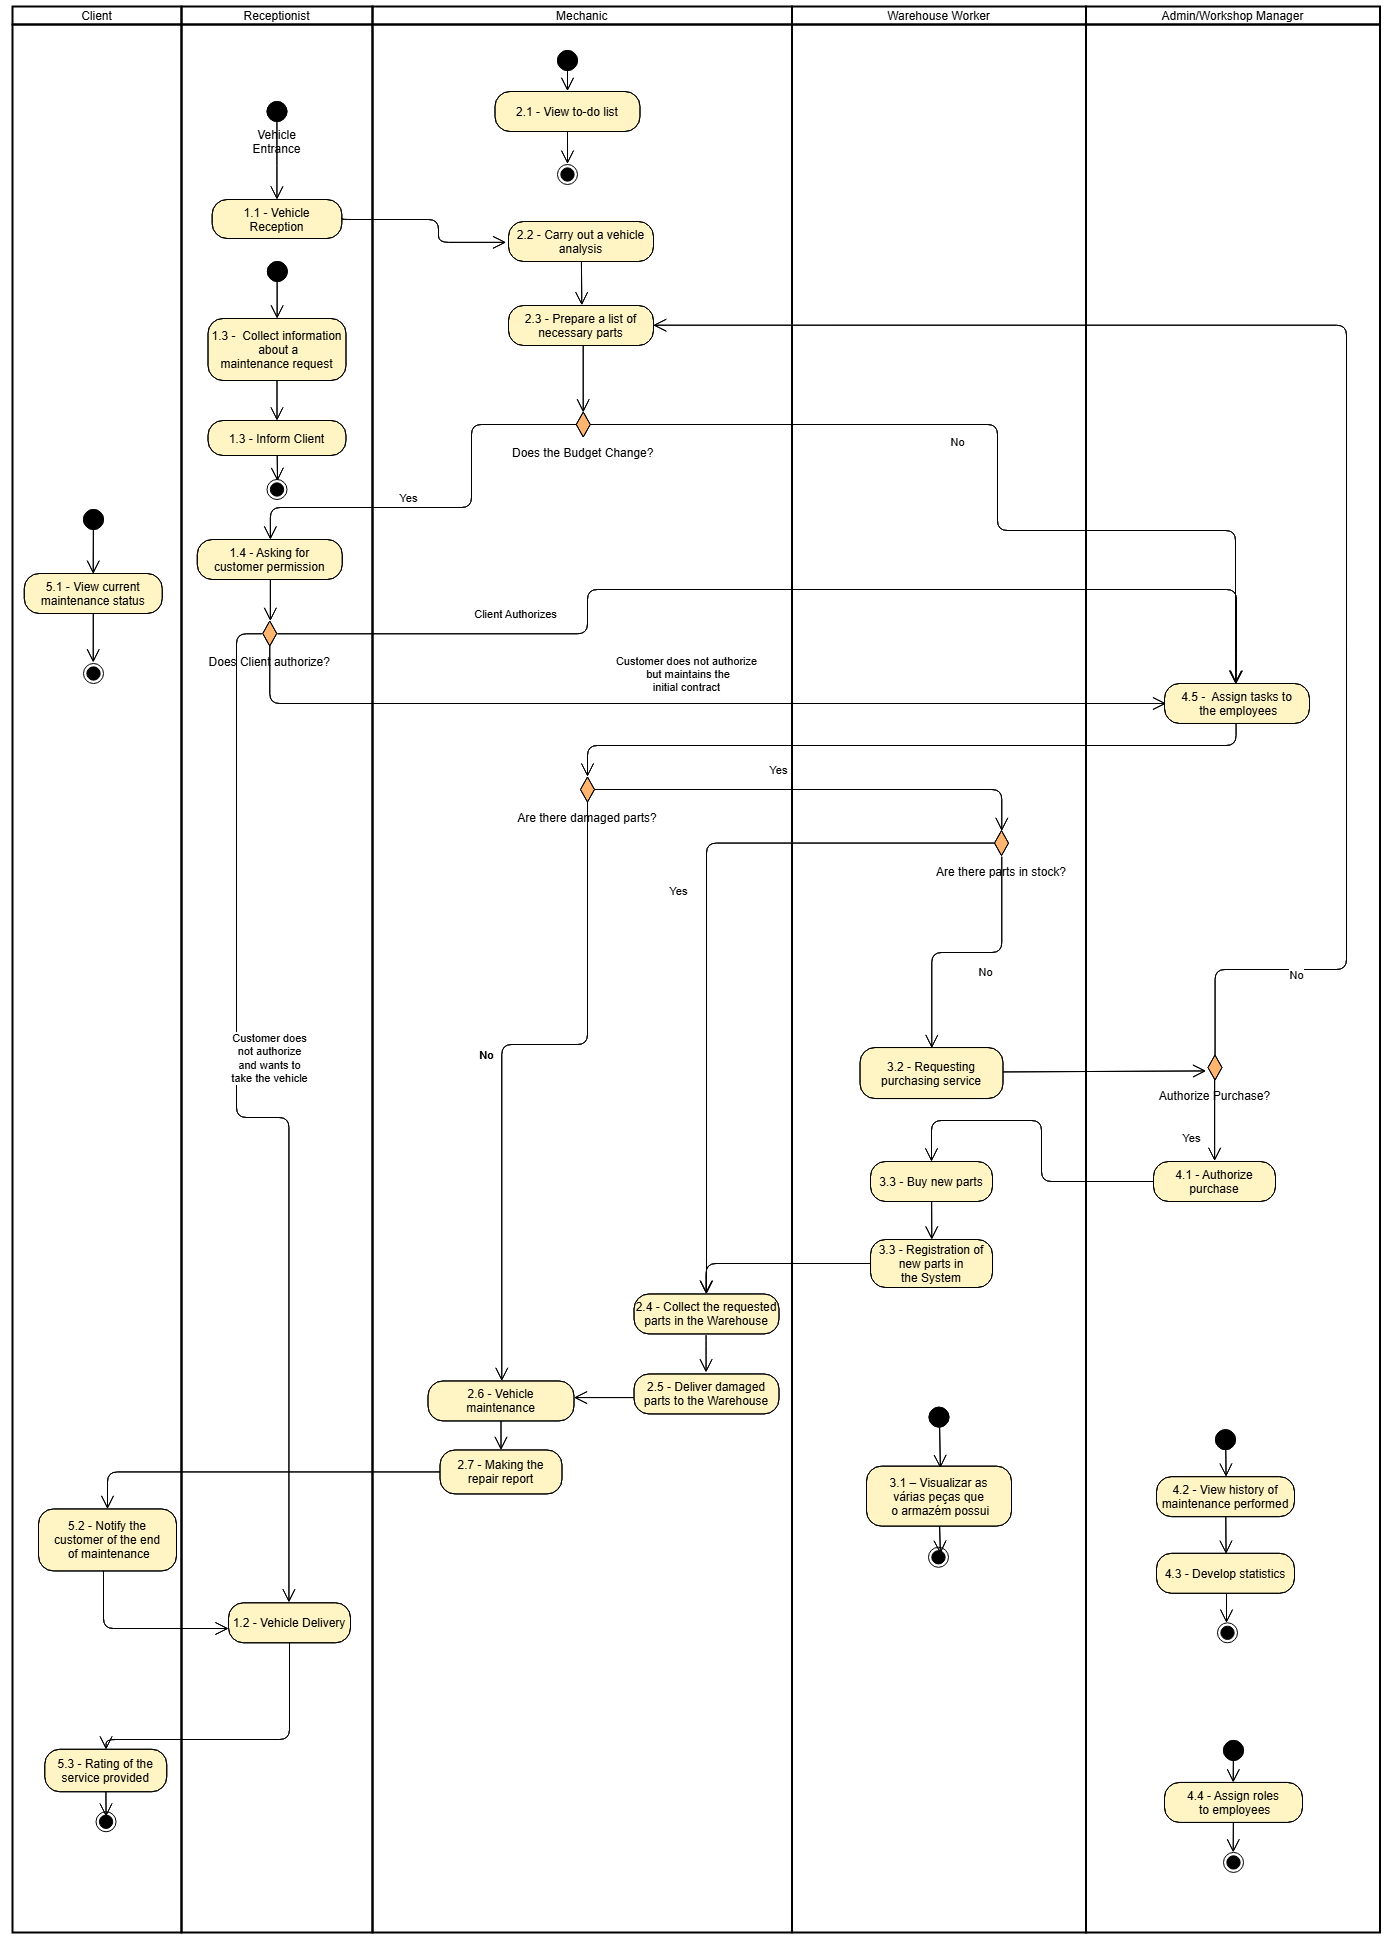
\includegraphics[width=\textwidth]{figs/UseCaseDiagram}
  \label{fig:figure2}
\end{figure}

The system's main flow starts when a Client arrives at the dealership for vehicle maintenance. 
The receptionist gets some input from the client and decides on an initial budget and check-out date agreed with him and inserts the information in the system (Use Case 1.1).
After that, a worker will be responsible for doing the analysis of the vehicle. 
He will add to the system all the problems he finds and the necessary parts that need to be replaced (Use Case 2.2 and 2.3).


If the budget to complete the work or the expected time changes, an alert is sent to the receptionist to inform the Client (Use Case 1.4). 
The result of this interaction must be "authorize the changes and continue the work", "not authorize the changes but continue as initially agreed" or "not authorizing the changes and wanting to check out the vehicle".
In the last case, the vehicle is delivered and the app will request the client to rate the service (Use Case 1.2 and 5.3). 
In any other case, the maintenance process continues. The only difference is the maintenance process information is alterated in the not authorized case.

After this step, the admin will receive a notification of the new tasks and will assign them to each worker (Use Case 4.5).
From there on, the maintenance process can or can not require the need for a vehicle part to be replaced. 
In the negative case the vehicle goes to the responsible mechanic to do the oil change, tire change, wash, etc (Use Case 2.6). 
In the affirmative case, the Warehouse Operator will check if the parts the mechanic requested are available in stock. 
If it does, the operator accepts the request and delivers the parts to the mechanic, who will replace the parts of the vehicle, deliver the damaged parts to the warehouse, and do the maintenance (Use Case 2.4, 2.5 and 2.6). 
If it does not, the operator needs to buy new parts from the supplier. 
In this case, he initiates a new requesting purchase that can be authorized by the admin. 
In the optimal case, the admin accepts the purchase, the operator buys the new parts, registers them in the system, and delivers them to the mechanic. 
In the worst scenario, the admin rejects the purchase and the mechanic needs to request new parts and restart the process (Use Case 2.3).    

Finally, when the vehicle maintenance is finished, the mechanic inserts into the system all operations and tests carried out as well as their results (Use Case 2.7). 
At once, the system notifies the customer that the vehicle is ready for the check out and, when the receptionist delivers the vehicle to the Customer, the client application asks to rate the system (Use Case 5.2, 1.2 and 5.3).

There are also a few secondary flows visible in the figure \ref{fig:figure2}. 
These flows are listed below:
\begin{itemize}
  \item The client enters the application to check the status of the maintenance (Use case 5.1);
  \item The mechanic enters the application to view the task he has to do (Use Case 2.1); 
  \item The Warehouse Operator enters the application to visualize the diverse parts and components in the warehouse (Use case 3.1); 
  \item The Admin enters the application to assign roles and/or permissions to the employees (Use Case 4.4); 
  \item The Admin enters the application to gather information about a maintenance performed and see statistics about that information (Use Case 4.2 and 4.3); 
\end{itemize}
 








